\chapter{Introducción Específica} % Main chapter title

\label{Chapter2}

%----------------------------------------------------------------------------------------
%	SECTION 1
En esta capítulo se detalla la plataforma de hardware utilizada, y se hace una introducción a la arquitectura del firmware y software.
%----------------------------------------------------------------------------------------
\section{La plataforma de Hardware}
\label{sec:plataforma}

La Computadora Industrial Abierta Argentina (CIAA) es un proyecto que comenzó en el año 2013 
gracias a la acción conjunta de \textit{ACSE}\footnote{ACSE: Asociación Civil para la investigación, promoción y desarrollo de los Sistemas electrónicos Embebidos.} y \textit{CADIEEL}\footnote{CADIEEL: Cámara Argentina de Industrias Electrónicas, Electromecánicas y Luminotécnicas.}, dando lugar a una plataforma de hardware que posee dos valiosas características: ser de carácter industrial, es decir, pensada y diseñada para las exigencias de confiabilidad que la industria requiere, y ser abierta bajo licencia BSD, lo cual promueve su uso, modificación y redistribución.

Este trabajo se basó principalmente en la versión educativa de esta computadora, llamada “EDU-CIAA-NXP” la cual utiliza un microcontrolador NXP LPC 4337 JDB 144 (Dual-core Cortex-M4 + Cortex-M0).

\begin{figure}[ht]
  \centering
    \includegraphics[width=0.7\textwidth]{Figures/fig_educiaa_diagrama_en_bloques}
  \caption{Diagrama en bloques de la plataforma EDU-CIAA-NXP}
  \label{fig:educiaaBloques}
\end{figure}

Como se observa en la figura \ref{fig:educiaaBloques} la placa tiene 4 pulsadores, 3 leds y un led RGB con los cuales es posible realizar muchos ejercicios, asi como tambien una conexión USB mediante un chip FT2232 el cual brinda un puerto JTAG y una UART para conectar el microcontrolador con la PC.
La placa también posee dos conectores P1 y P2 de 40 pines cada uno, en donde se encuentran conectados los periféricos del micontrontrolador (GPIOs, UARTs, SPI, I2C, etc.)


\begin{figure}[ht]
  \centering
    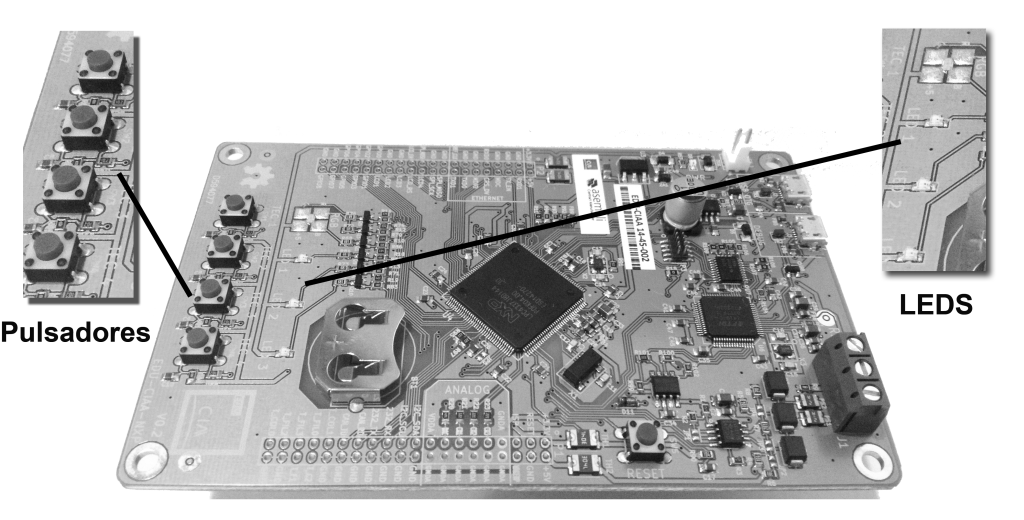
\includegraphics[width=0.7\textwidth]{Figures/fig_educiaa_placa}
  \caption{Foto de una placa EDU-CIAA-NXP}
  \label{fig:educiaaPlaca}
\end{figure}

El diseño fue pensado para proveer una plataforma de desarrollo moderna y económica basada en la CIAA que sirva a docentes y a estudiantes en los cursos de sistemas embebidos y lograr una amplia inserción en el sistema educativo argentino.

En la figura \ref{fig:educiaaPlaca} se muestra una foto de una placa EDU-CIAA-NXP en donde se puede observar claramente los 4 pulsadores y los leds SMD que permiten realizar ejercicios sin requerir componentes adicionales.

%----------------------------------------------------------------------------------------

\section{Utilización de MicroPython}
\label{sec:micropython}

El proyecto MicroPython \cite{micropython} es un desarrollo de firmware realizado por Damien George, el cual fue pensado para correr sobre la plataforma Pyboard, desarrollada por Jaltek Systems \cite{jaltek}. Este proyecto permite la ejecución de código Python y la utilización de los periféricos que posee la placa, desde dicho lenguaje.

\begin{figure}[ht]
  \centering
    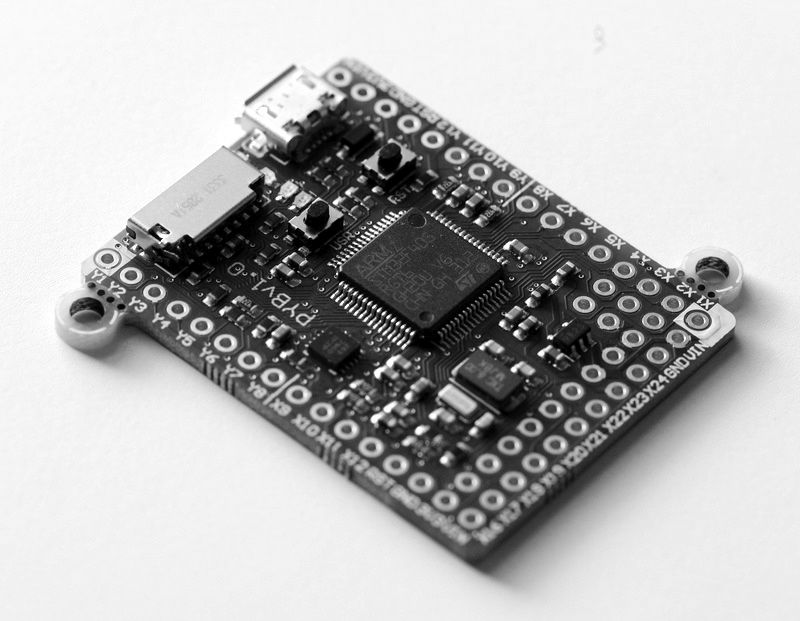
\includegraphics[width=0.4\textwidth]{Figures/fig_pyboard}
  \caption{Foto de una placa Pyboard}
  \label{fig:pyboardPlaca}
\end{figure}

Las características del microcontrolador que posee esta placa, son similares a las de la EDU-CIAA-NXP (Cortex-M4@168Mhz).

Para obtener la capacidad de ejecutar código Python en la EDU-CIAA-NXP, se adoptó el trabajo de Martin Ribelotta, quien realizó el port del proyecto MicroPython mencionado previamente para esta plataforma \cite{portmicropythonribelotta}.
Este port constaba de la inicialización del intérprete, el cual permitía ejecutar código Python, la inicialización y configuración de la \textit{Garbage Collector}\footnote{Garbage Collector: Gestor automático de memoria dinámica.} y la implementación de un filesystem FAT12 embebido en la memoria de programa del microcontrolador, de manera de poder escribir en forma permanente el código Python en la memoria y luego ser ejecutado desde allí. 

%El port no contaba con la implementación para el manejo de los periféricos del microcontrolador, el autor comenzó a desarrollar el soporte para algunos periféricos antes de dar comienzo a este trabajo, dicho soporte se tomó como punto de partida y se reescribió y mejoró en gran medida para lograr la calidad del firmware deseada al implementar técnicas de ingeniería de software.

El autor del presente trabajo comenzó a desarrollar el soporte para algunos periféricos a mediados de 2015, ya que el port de Martin Ribelotta no contaba con la implementación para el manejo de dichos periféricos. Esto se tomó como punto de partida y se reescribió y mejoró en gran medida para lograr la calidad del firmware deseada al implementar técnicas de ingeniería de software.
%----------------------------------------------------------------------------------------

\section{Arquitectura del Firmware}
\label{sec:firmwareArq}

A continuación se detallará la arquitectura del firmware implementado en este trabajo. En la misma se pueden apreciar los siguientes bloques:

\begin{itemize}
	\item \textbf{EDU-CIAA-NXP}: representa el hardware donde se ejecuta el firmware.
	\item \textbf{Intérprete uPython}: representa el código del proyecto MicroPython, mediante el cual es posible interpretar y ejecutar el código Python escrito por el usuario.
	\item \textbf{Código Python programado por el usuario}: representa el código que el usuario escribe en el IDE y graba en la placa para su posterior ejecución.
\end{itemize}

\begin{figure}[ht]
  \centering
    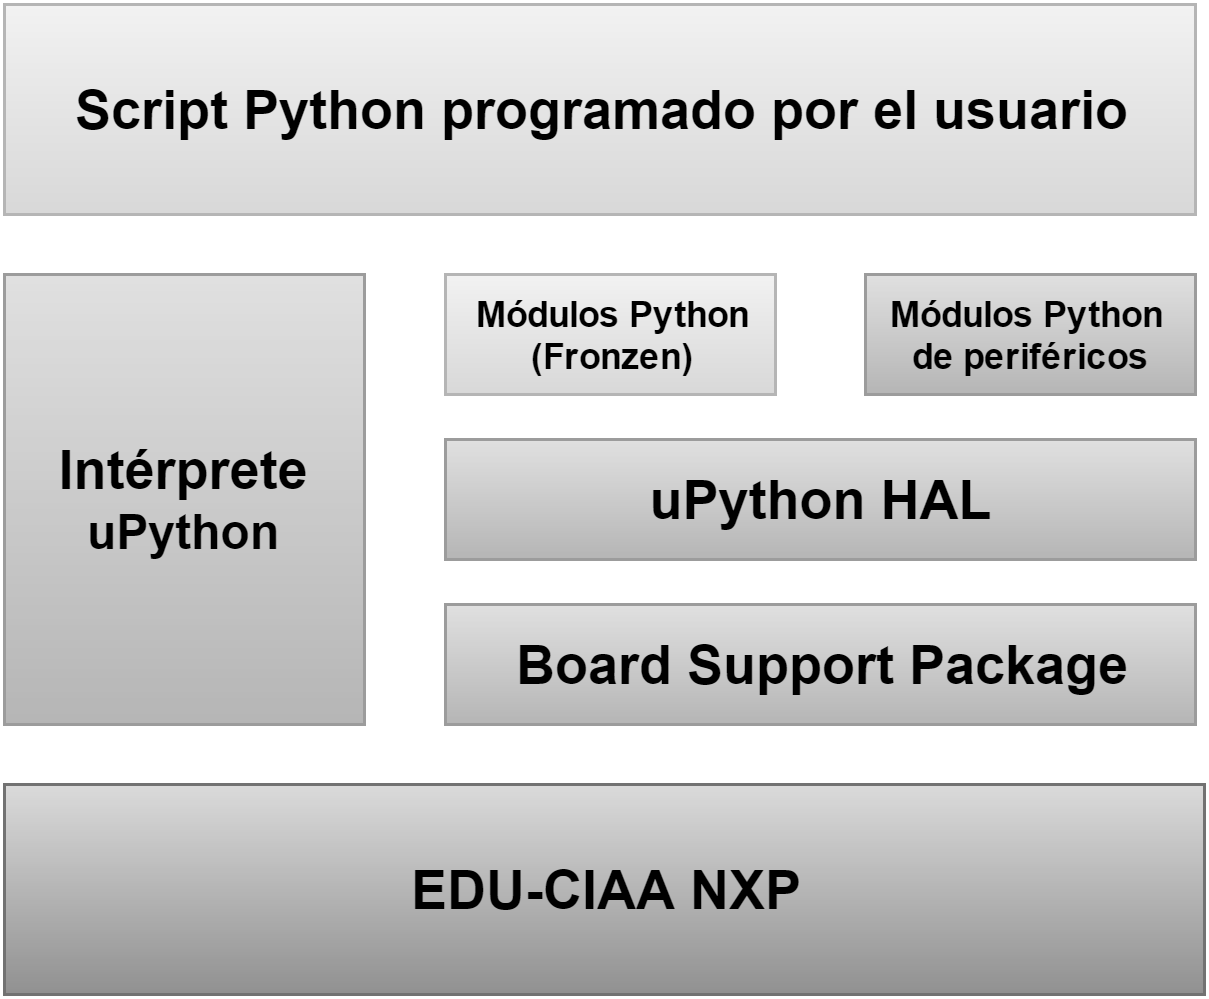
\includegraphics[width=0.7\textwidth]{Figures/fig_firm_arquitectura}
  \caption{Diagrama en bloques de la arquitectura del Firmware}
  \label{fig:firmwareArq}
\end{figure}

Estos tres bloques mencionados y que pueden identificarse en la figura \ref{fig:firmwareArq} representan el firmware del proyecto MicroPython creado por Martin Ribelotta que se tomó como punto de partida para el desarrollo de este trabajo. 

A continuación se detallan los bloques que se han desarrollado:

\begin{itemize}
	\item \textbf{Board Support Package}: aquí se encuentra la biblioteca que permite el acceso, uso e inicialización de los periféricos del microcontrolador.
	\item \textbf{uPython HAL}: capa de abstracción del hardware. El proyecto MicroPython utiliza esta capa para abstraer funciones específicas del hardware y que el código que utilice los periféricos sea portable.
	\item \textbf{Módulos Python de periféricos}: para que el usuario pueda utilizar los periféricos desde el código Python, se necesita escribir un código en lenguaje C que represente una clase Python, en dicho código se consigue ejecutar funciones de C al ejecutar funciones de Python, de esta manera se logra utilizar la capa uPython HAL desde el código Python escrito por el usuario.
	\item \textbf{Módulos Python (Frozen)}: también es posible escribir bibliotecas Python directamente en lenguaje Python, y que las mismas formen parte del firmware. Este trabajo incluyó una biblioteca escrita en Python que permite la ejecución de tests unitarios.
\end{itemize}

%----------------------------------------------------------------------------------------

\section{Arquitectura del Software}
\label{sec:softwareArq}

A continuación se detallará la arquitectura del entorno de desarrollo, en la cual se describe la utilización de una ventana principal en donde se puede editar el archivo de código Python, y mediante un mecanismo de plug-ins se indica la incorporación de ventanas específicas que tienen que ver con el proceso de grabar el código en la EDU-CIAA-NXP. 

\begin{figure}[ht]
  \centering
    \includegraphics[width=0.8\textwidth]{Figures/fig_soft_arquitectura}
  \caption{Diagrama en bloques de la arquitectura del Software del IDE}
  \label{fig:softwareArq}
\end{figure}

En la figura \ref{fig:softwareArq} se observan los siguientes módulos de software que componen el IDE:

\begin{itemize}
	\item \textbf{Archivo .py}: representa el archivo que se abre, edita y guarda usando el IDE. En este archivo se escribirá el código Python que se grabará y ejecutará en la placa.
	\item \textbf{Editor de archivo .py}: representa la capa gráfica del programa en donde se escribe el código Python.
	\item \textbf{Lógica del editor}: representa las funciones que permiten que la ventana principal donde se escribe el código funcione como un editor de texto.
	\item \textbf{Sistema de plug-ins}: la lógica del editor incorpora un sistema de plug-ins mediante el cual se agregan opciones al menú y permiten ejecutar ventanas adicionales a la principal.
	\item \textbf{Menú para la EDU-CIAA-NXP}: aquí se encuentran las opciones que permiten interactuar con la placa y los ejemplos.
\end{itemize}

Dentro de las ventanas agregadas, se encuentran las que permiten la grabación del código en la placa, la ejecución de una terminal serial, mediante la cual es posible visualizar el standard output del código Python e ingresar datos por el standard input, una ventana con una lista de porciones de código de ejemplo (Snippets) y una ventana de configuración en donde se declara el puerto serie de la PC a utilizar.
A continuación se detallan los módulos de software correspondientes a las ventanas mencionadas previamente:

\begin{itemize}
	\item \textbf{Ventana de configuración}: aquí se permite elegir el puerto serie de la PC en donde se conectó la placa.
	\item \textbf{Lógica configuración}: representa las funciones que manejan la ventana de configuración.
	\item \textbf{Ventana de grabación}: aquí se muestra el progreso del envío del archivo a la placa.
	\item \textbf{Lógica de grabación}: representa las funciones que se encargan de enviar el archivo a la placa y mostrar el progreso en la ventana de grabación.
	\item \textbf{Ventana de Snippets}: aquí se muestra una lista de porciones de código de ejemplo y mediante un botón se puede agregar dicha porción de código al archivo que se está escribiendo.
	\item \textbf{Lógica de Snippets}: representa las funciones que manejan la interacción del usuario con la ventana de Snippets.
	\item \textbf{Ventana terminal serie}: aquí se muestra el stdout del código de Python que se ejecuta en la placa y se capturan las teclas que presiona el usuario y se envian hacia el stdin del código Python que se ejecuta en la placa.
	\item \textbf{Lógica terminal serie}: representa las funciones encargadas de la comunicación serie y representación en la ventana.
\end{itemize}
	
El desarrollo de este IDE se basó en el IDE del proyecto EDILE \cite{edile}, y se agregaron las ventanas específicas mencionadas previamente.





%----------------------------------------------------------------------------------------


\section{Requerimientos}
\label{sec:req}

A continuación se detallan los requerimientos planteados para la realización de este trabajo.

Grupo de requerimientos referidos a las bibliotecas Python:
\begin{enumerate}
	\item  Manejo de los leds que dispone la placa.
	\item  Utilización de los pulsadores.
	\item  Manejo y configuración de los pines designados como GPIO. 
	\item  Configuración y utilización de la UART.
	\item  Configuración y utilización de la interface RS485.
	\item  Lectura de las entradas ADC.
	\item  Salida DAC.
	\item  Utilización de la EEPROM interna.
	\item  Utilización de Timers.
\end{enumerate}

Grupo de requerimientos referidos al entorno de desarrollo:
\begin{enumerate}
	\item  El software deberá ser multiplataforma (Windows/Linux/OSX).
	\item  No debe ser necesario recompilar el firmware de la placa para cambiar el código de python.
	\item  El programa de python se enviará por el COM virtual generado al conectar la placa a la PC. 
	\item  El software deberá tener embebida una terminal serial, por donde se implementará la interfaz de salida y entrada estándar del programa de Python. 
	\item  El software deberá tener porciones de código de ejemplo que puedan insertarse fácilmente junto con lo que el usuario programa (Snippets)
	\item  El software deberá tener links para acceder fácilmente a la documentación online y a los proyectos de ejemplo.
\end{enumerate}

Grupo de requerimientos referidos a los proyectos de ejemplo:
\begin{enumerate}
	\item  Los proyectos de ejemplo serán divididos en tres categorías: Inicial, Intermedio y Avanzado. 
	\item  Los proyectos de ejemplo consistirán en el código fuente, la explicación del mismo en forma detallada, y un esquemático de conexión con componentes externos en el caso que se requiera.
	\item  Los proyectos de ejemplo están basados en los proyectos típicos de electrónica que se realizan en escuelas secundarias. 
\end{enumerate}

Grupo de requerimientos generales:
\begin{enumerate}
	\item  El acceso a la información del proyecto será libre y gratuita.  
	\item  Se publicará la documentación de las bibliotecas de Python disponibles para programar.
\end{enumerate}


%----------------------------------------------------------------------------------------


